\section{Results}

%\begin{figure}
%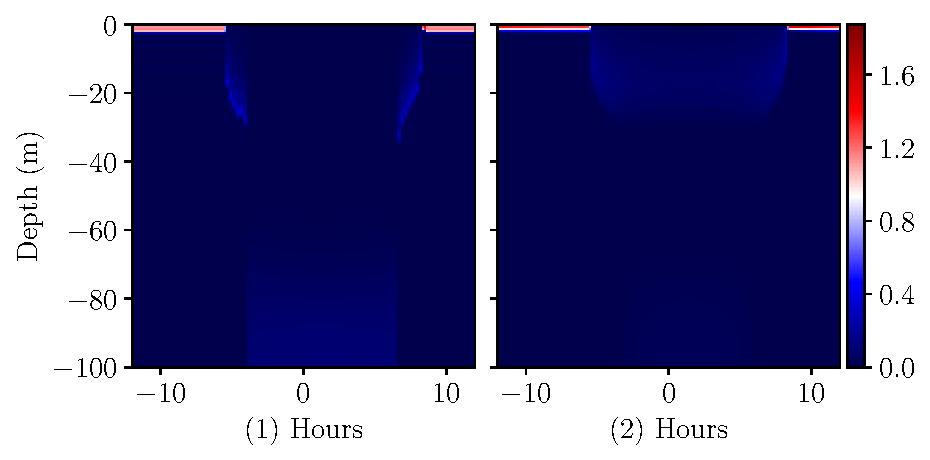
\includegraphics{heatmapsday10_nonrandom.pdf}
%\caption{Vertical distribution of consumers \emph{(1)} and predators \emph{(2)} throughout the 1st of May, in hours from noon.}
%\end{figure}

\begin{figure}
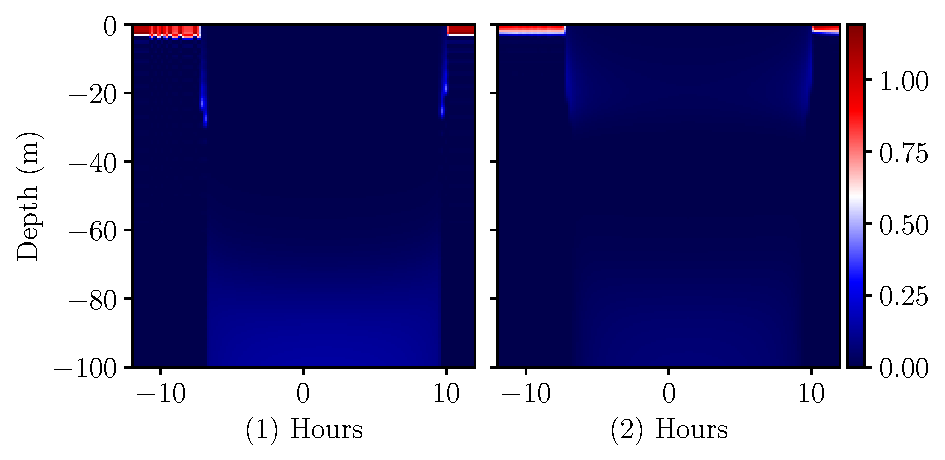
\includegraphics{heatmapsday90_nonrandom.pdf}
\caption{Vertical distribution of consumers \emph{(1)} and predators \emph{(2)} throughout the 1st of July. The time is in hours from noon. }
\label{fig:heatmaps_90_nonrandom}
\end{figure}
The vertical migration of consumers, \Cref{fig:heatmaps_90_nonrandom}(1) is clear here in the middle of the summer.They are highly concentrated at the top of the water column during nighttime, and at day they scatter throughout the deep. The pattern of the predators is slightly different from the consumer pattern, \Cref{fig:heatmaps_90_nonrandom}. At nighttime there is still a non-zero concentration of predators in the upper layers of the water-column, there to catch any errant prey.
\begin{figure}
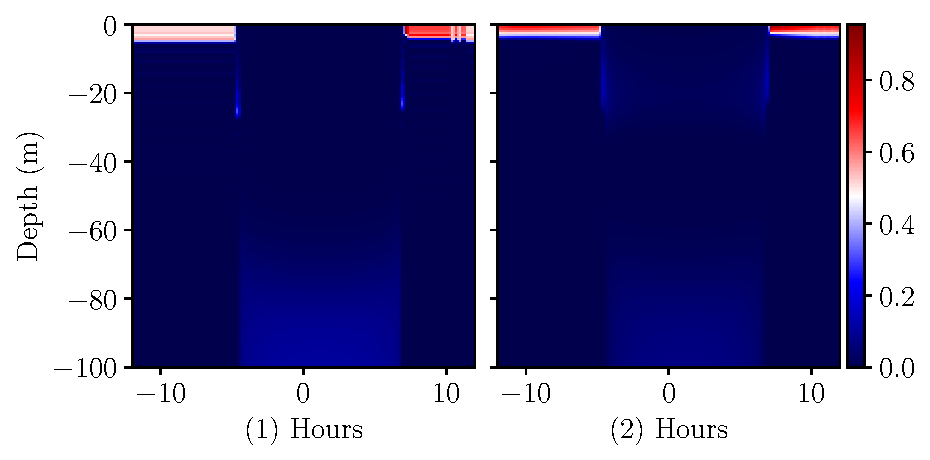
\includegraphics{heatmapsday180_nonrandom.pdf}
\caption{Vertical distribution of consumers \emph{(1)} and predators \emph{(2)} throughout the 1st of October. The time is in hours from noon.}
\label{fig:heatmaps_180_nonrandom}
\end{figure}
Moving the hands on the clock forward to October, we again see a clearly defined vertical migration, \Cref{fig:heatmaps_180_nonrandom}. The migration differs from the previous migration, in that the descent and ascent are steeper, and the distributions are wider during the night.

\begin{figure}
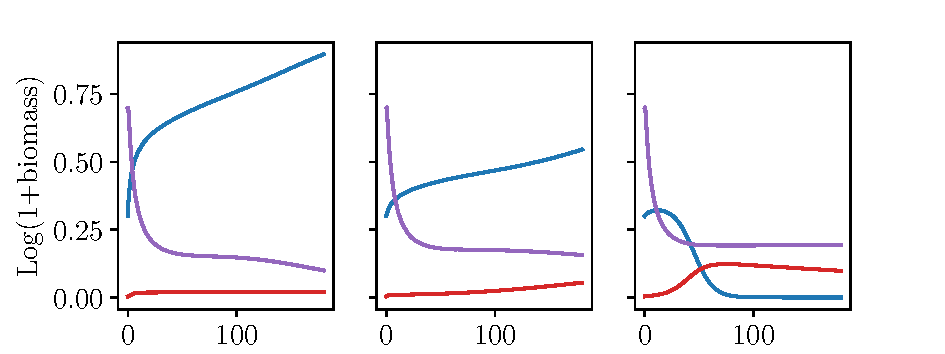
\includegraphics{populations.pdf}
\caption{Total populations of consumers \emph{(blue)}, predators, \emph{(red)} and resources \emph{(purple)} from 1st of april to 1st of october. We vary the rationality, from total rationality \emph{(1)}, bounded rationality ($\sigma = 10...$), \emph{(2)} and fully irrational, $\sigma = \infty$, \emph{(3)}.}
\label{fig:long_term_populations}
\end{figure}
The the difference in population dynamics between a system with no behavioral optimization, \Cref{fig:long_term_populations}(3), bounded rationality \Cref{fig:long_term_populations}(2) and full rationality \Cref{fig:long_term_populations}(1) is stark. The resources reach a stable level quickly in all three cases, but the populations of consumers and predators differ markedly. The difference in populations between the system with bounded rationality \Cref{fig:long_term_populations}(2) and the fully rational system appears to be negligible, \Cref{fig:long_term_populations}(1). The main driver seems to be the ability to retreat to a refuge, and not exactly how it happens.
%Large differences between irrational and the rational possibilities
\begin{figure}
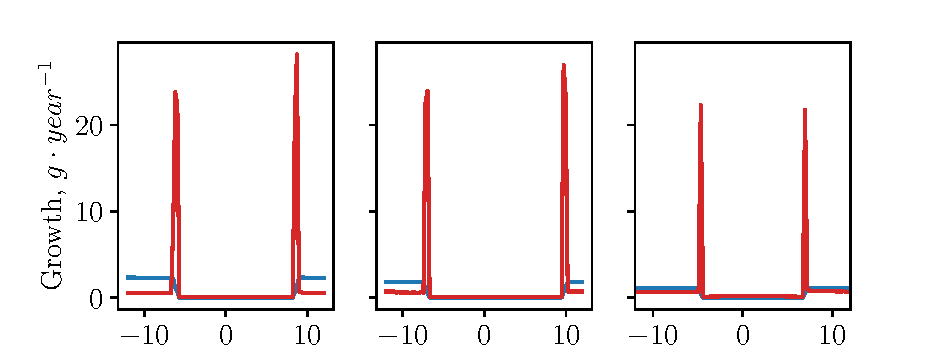
\includegraphics{growth_short_rational.pdf}
\caption{Seasonal comparison of consumer \emph{(blue)} and predator, \emph{(red)} feeding patterns on 1st of May \emph{(1)}, 1st of July \emph{(2)} and 1st of October \emph{(3)}}
\end{figure}

\begin{figure}
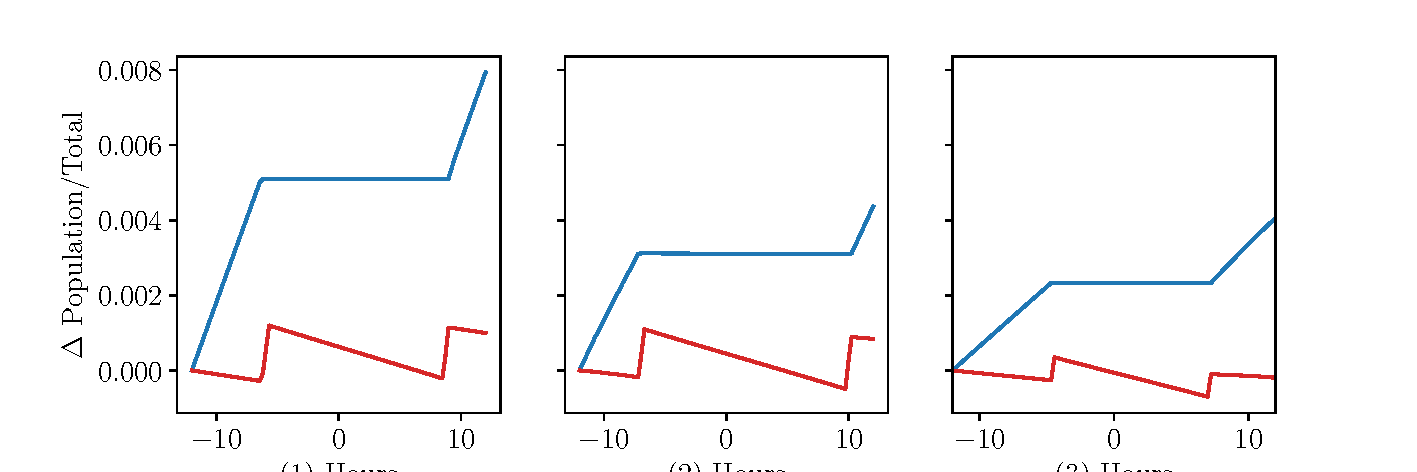
\includegraphics{pop_short_rational.pdf}
\caption{Seasonal comparison of consumer \emph{(blue)} and predator, \emph{(red)} pr. capita growth patterns on 1st of May \emph{(1)}, 1st of July \emph{(2)} and 1st of October \emph{(3)}}
\label{fig:pop_short_term}

\end{figure}
Clear emergence
\begin{figure}
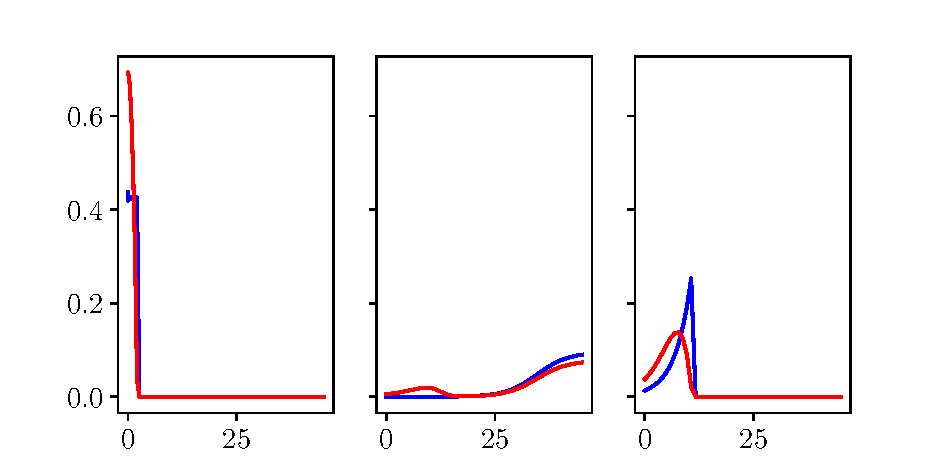
\includegraphics{specific_dists_rational.pdf}
\caption{Daily distribution of consumers \emph{blue} and predators \emph{red} at midnight \emph{(1)}, noon \emph{(2)} and at 18:45, \emph{3} with full rationality}
\label{fig:specific_dists_rational}
\end{figure}

Tracking, preventive
\begin{figure}
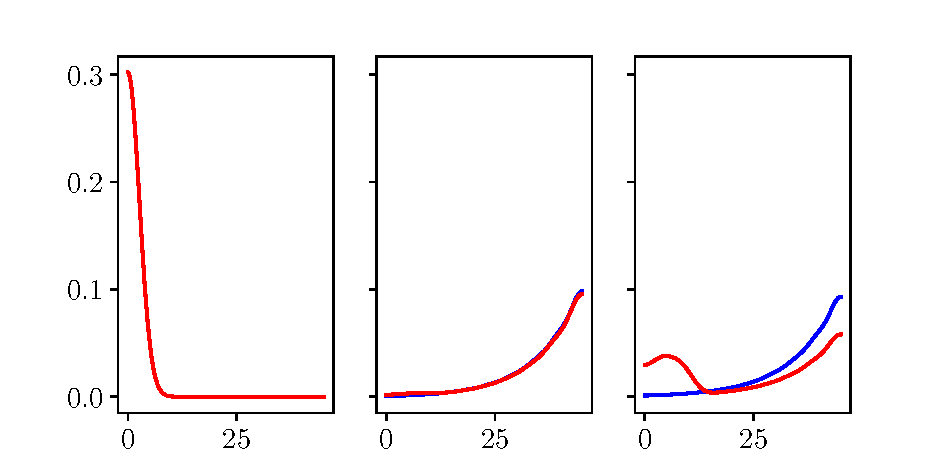
\includegraphics{specific_dists_semirational.pdf}
\caption{Daily distribution of consumers \emph{blue} and predators \emph{red} at midnight \emph{(1)}, noon \emph{(2)} and at 18:45, \emph{(3)} with bounded rationality}
\label{fig:specific_dists_irrational}
\end{figure}

Smoother, more realistic
